\documentclass[
  bibliography=totoc,     % Literatur im Inhaltsverzeichnis
  captions=tableheading,  % Tabellenüberschriften
  titlepage=firstiscover, % Titelseite ist Deckblatt
]{scrartcl}

% Paket float verbessern
\usepackage{scrhack}

%csv Dateien einlesen
\usepackage{csvsimple}

% Warnung, falls nochmal kompiliert werden muss
\usepackage[aux]{rerunfilecheck}

% unverzichtbare Mathe-Befehle
\usepackage{amsmath}
% viele Mathe-Symbole
\usepackage{amssymb}
% Erweiterungen für amsmath
\usepackage{mathtools}

% Fonteinstellungen
\usepackage{fontspec}
% Latin Modern Fonts werden automatisch geladen
% Alternativ zum Beispiel:
%\setromanfont{Libertinus Serif}
%\setsansfont{Libertinus Sans}
%\setmonofont{Libertinus Mono}

% Wenn man andere Schriftarten gesetzt hat,
% sollte man das Seiten-Layout neu berechnen lassen
\recalctypearea{}

% deutsche Spracheinstellungen
\usepackage[main=ngerman]{babel}


\usepackage[
  math-style=ISO,    % ┐
  bold-style=ISO,    % │
  sans-style=italic, % │ ISO-Standard folgen
  nabla=upright,     % │
  partial=upright,   % ┘
  warnings-off={           % ┐
    mathtools-colon,       % │ unnötige Warnungen ausschalten
    mathtools-overbracket, % │
  },                       % ┘
]{unicode-math}

% traditionelle Fonts für Mathematik
\setmathfont{Latin Modern Math}
% Alternativ zum Beispiel:
%\setmathfont{Libertinus Math}

\setmathfont{XITS Math}[range={scr, bfscr}]
\setmathfont{XITS Math}[range={cal, bfcal}, StylisticSet=1]

% Zahlen und Einheiten
\usepackage[
  locale=DE,                   % deutsche Einstellungen
  separate-uncertainty=true,   % immer Fehler mit \pm
  per-mode=symbol-or-fraction, % / in inline math, fraction in display math
]{siunitx}

% chemische Formeln
\usepackage[
  version=4,
  math-greek=default, % ┐ mit unicode-math zusammenarbeiten
  text-greek=default, % ┘
]{mhchem}

% richtige Anführungszeichen
\usepackage[autostyle]{csquotes}

% schöne Brüche im Text
\usepackage{xfrac}

% Standardplatzierung für Floats einstellen
\usepackage{float}
\floatplacement{figure}{htbp}
\floatplacement{table}{htbp}

% Floats innerhalb einer Section halten
\usepackage[
  section, % Floats innerhalb der Section halten
  below,   % unterhalb der Section aber auf der selben Seite ist ok
]{placeins}

% Seite drehen für breite Tabellen: landscape Umgebung
\usepackage{pdflscape}

% Captions schöner machen.
\usepackage[
  labelfont=bf,        % Tabelle x: Abbildung y: ist jetzt fett
  font=small,          % Schrift etwas kleiner als Dokument
  width=0.9\textwidth, % maximale Breite einer Caption schmaler
]{caption}
% subfigure, subtable, subref
\usepackage{subcaption}

% Grafiken können eingebunden werden
\usepackage{graphicx}
% größere Variation von Dateinamen möglich
\usepackage{grffile}

% schöne Tabellen
\usepackage{booktabs}

% Verbesserungen am Schriftbild
\usepackage{microtype}

% Literaturverzeichnis
\usepackage[
  backend=biber,
]{biblatex}
% Quellendatenbank
\addbibresource{lit.bib}
\addbibresource{programme.bib}

% Hyperlinks im Dokument
\usepackage[
  german,
  unicode,        % Unicode in PDF-Attributen erlauben
  pdfusetitle,    % Titel, Autoren und Datum als PDF-Attribute
  pdfcreator={},  % ┐ PDF-Attribute säubern
  pdfproducer={}, % ┘
]{hyperref}
% erweiterte Bookmarks im PDF
\usepackage{bookmark}

% Trennung von Wörtern mit Strichen
\usepackage[shortcuts]{extdash}
\author{%
  Samuel Haefs\\%
  \href{mailto:samuel.haefs@tu-dortmund.de}{samuel.haefs@tu-dortmund.de}%
  \and%
  Max Koch\\%
  \href{mailto:max.koch@tu-dortmund.de}{max.koch@tu-dortmund.de}%
}
\publishers{TU Dortmund – Fakultät Physik}

\subject{802}
\title{Fourier Synthese}
\date{%
  Durchführung: 22.10.2019
  \hspace{3em}
  Abgabe: 29.10.2019
}

\begin{document}

\maketitle
\thispagestyle{empty}
\tableofcontents
\newpage
%\printbibliography{}
\newpage
\section{Theorie}
Jede periodische Funktion läßt sich in eine Reihe aus sin- und cos-Termen entwickeln (Fourierreihe)
\begin{equation}
  f(t)=\sum_{i=0}^\infty (A_k\cdot cos(\omega_k t) + B_k\cdot sin(\omega_k t))
\end{equation}
mit
\begin{equation}
\omega_k=\frac{2\pi k}{T}
\label{eqn:omega}
\end{equation}
\section{Fourier-Zerlegung der Funktion |sin(x)|}
\subsection{Berechnung der Integrale}
Im folgenden soll die Funktion $f(x)=|sin(x)|$ mit einer Fourierreihe angenähert werden.
Die Koeffizienten sind definiert als
\begin{equation}
A_k=\frac{2}{T} \int_{-T/2}^{T/2} f(t) \cdot cos(\omega_k \cdot t)  \, \symup{d}t
\end{equation}
\begin{equation}
B_k=\frac{2}{T} \int_{-T/2}^{T/2} f(t) \cdot sin(\omega_k \cdot t)  \, \symup{d}t
\end{equation}
Die Funktion $|sin(x)|$ erfüllt die Eigenschaft $f(-x) = f(x)$ und ist somit eine gerade Funktion.
Somit ist unser $B_k=0$. 
Zunächst wählen wir $T=2\pi$. Somit ist $\omega_k =k$.
Daraus folgt für $A_k$
\begin{equation}
A_k=\frac{1}{\pi} \int_{-\pi}^{\pi} |sin(t)| \cdot cos(\omega_k \cdot t) \, \symup{d}t
\end{equation}
Die Funktion $|sin(x)|$ ist $\pi$-periodisch und hat bei $x = 0$ eine Nullstelle.
Wir integrieren nun über eine, statt wie zuvor über zwei Perioden. Es gilt 
$\int_{-\pi}^{0}f(x) \, \symup{d}x = \int_0^{\pi} f(x) \, \symup{d}x$
erhalten wir zusätlich einen Faktor $2$.
\begin{equation}
A_k=\frac{2}{\pi} \int_0^{\pi} |sin(t)| \cdot cos(\omega_k \cdot t) \, \symup{d}t
\end{equation}
Es gilt $|sin(x)| = sin(x)$ im Intervall $I=[0,\pi]$, so können wir
unser Integral vereinfachen
\begin{equation}
A_k=\frac{2}{\pi} \int_0^{\pi} sin(t) \cdot cos(\omega_k \cdot t)  \, \symup{d}t
\end{equation}
\begin{equation}
\Rightarrow A_k= \frac{2}{\pi} \left [ \frac{cos((\omega_k-1)t)}{2(w-1)} - \frac{cos((\omega_k+1)t)}{2(\omega_k^2+1)} \right ]_0^{\pi}
\end{equation}
mit $\omega_k$ und Grenzen eingesetzt erhalten wir
\eqref{eqn:omega}
\begin{equation}
A_k=\frac{2}{\pi}\left ( \frac{cos(2k\pi-\pi)}{4k-2} - \frac{cos(2k\pi+\pi)}{4k+2} - \frac{cos(0)}{4k-2} + \frac{cos(0)}{4k+2} \right )
\end{equation}
\begin{equation}
\Leftrightarrow A_k=\frac{2}{\pi}\left ( \frac{-1}{4k-2} + \frac{1}{4k+2} - \frac{1}{4k-2} + \frac{1}{4k+2} \right )
\end{equation}
\begin{equation}
\Leftrightarrow A_k= \frac{2}{\pi} \left ( \frac{-8}{(4k-2)(4k+2)} \right )
\end{equation}
\begin{equation}
\Leftrightarrow A_k= \frac{4}{-4k^2 \pi + \pi}
\end{equation}
\subsection{Tabelle}
Für das online-Experiment werden 17 Koeffizienten benötigt um die
Regler einzustellen 
%tabelle
\begin{table}
  \centering
  \label{tab:koeffizienten}
  \begin{tabular}{c c}
    \toprule
    $k$ & $A_k$\\
    \midrule
      0 & 1.27323954e+00\\
      1 & -4.24413182e-01\\ 
      2 & -8.48826363e-02\\ 
      3 & -3.63782727e-02\\
      4 & -2.02101515e-02\\
      5 & -1.28610055e-02\\ 
      6 & -8.90377304e-03\\
      7 & -6.52943356e-03\\
      8 & -4.99309625e-03\\
      9 & -3.94191810e-03\\
      10 & -3.19107655e-03\\
      11 & -2.63610672e-03\\
      12 & -2.21432964e-03\\
      13 & -1.88628081e-03\\
      14 & -1.62610414e-03\\
      15 & -1.41628425e-03\\
      16 & -1.24461344e-03\\
      17 & -1.10237190e-03\\
    \bottomrule
  \end{tabular}
\end{table}
\newpage
\subsection{Plot}
Wir erhalten als Ergebnis auf der
\href{https://www.j-berkemeier.de/Fouriersynthese.html}{Website}
folgende Grafik
\begin{figure}
  \centering
  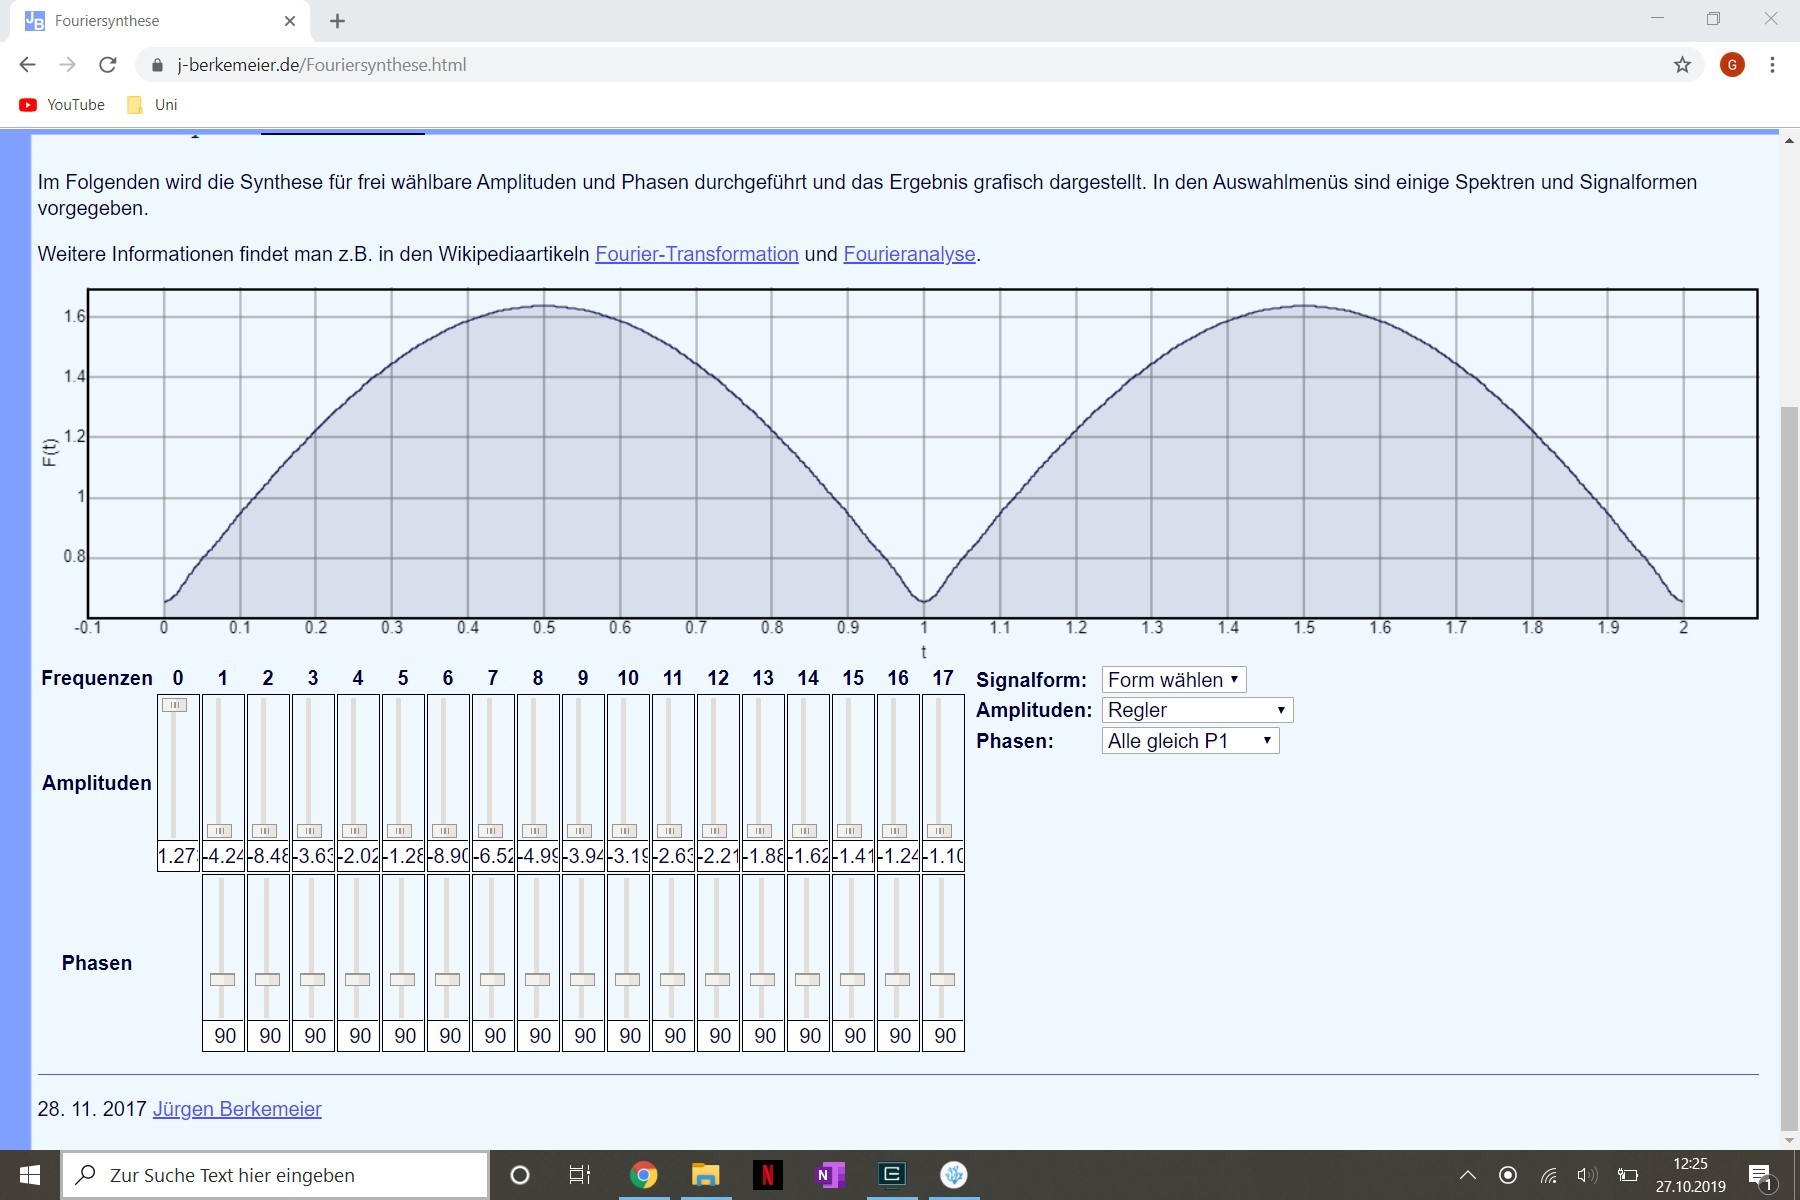
\includegraphics[height=10cm]{content/screenshot_phase90}
  \caption{Fouriersynthese von $|sin(x)|$}
  \label{fig:sin}
\end{figure}
\section{Fourier-Zeregung der Funktion f(x)=x}
    Im folgenden soll die Funktion $f(x)=|x|$ für $-pi < x < pi$ mit einer Fourierreihe angenähert werden.
    Die Koeffizienten sind definiert als
\newpage
\begin{equation}
  A_k=\frac{2}{T} \int_{-T/2}^{T/2} f(t) \, cos(\omega_k \, t) \,  dt
\end{equation}
\begin{equation}
  B_k=\frac{2}{T} \int_{-T/2}^{T/2} f(t) \, sin(\omega_k \, t) \, dt
\end{equation}
  Zunächst wird der Koeffizient $A_k$ berechnet, dafür $t$  $-\pi < t < \pi$ gilt, ist $T = 2\pi$
\begin{equation}
  A_k = \frac{1}{\pi} \int_{-\pi}^{\pi} t cos(\omega_k\, t) dt
\end{equation}
  Durch eine partielle Integration ergibt sich für $A_k$
\begin{equation}
  A_k= \frac{1}{\pi} \left [\frac{sin(\omega_k \, t)}{\omega_k} + \frac{cos(\omega_k \, t)}{\omega_k^2}  \right]_{-\pi}^{\pi} 
\end{equation}
  Nach einsetzten der Grenzen ergibt sich für $A_k$
\begin{equation}
  A_k = \frac{2 \, sin(\pi k)}{\omega_k} = 0
\end{equation}
  Nun zu $B_k$
\begin{equation}
  B_k = \frac{1}{\pi} \int_{-\pi}^{\pi} t \, sin (\omega_k t) \, dt
\end{equation}
  Durch eine partielle Integration ergibt sich für $B_k$
\begin{equation}
  B_k = \frac{1}{\pi} \left [\frac{- t \, cos(\omega_k \,  t)}{\omega} + \frac{sin(\omega_k t)}{\omega_k^2}\right]_{-\pi}^{\pi} 
\end{equation}
  Nach einsetzten der Grenzen fällt die sinus Funktion und für $B_k$ ergibt sich
\begin{equation}
  B_k = \frac{-2 \, (-1)^k}{k}
\end{equation}
Damit ergeben sich folgende Werte für den Koeffizient $B_k$
\begin{table}
  \centering
  \label{tab:koeffizienten}
  \begin{tabular}{c c}
    \toprule
    $k$ & $A_k$\\
    \midrule
    0 &0 \\
    1 &-1.0 \\
    2 &0.6666666666666666\\
    3 &-0.5\\
    4 &0.4\\
    5 &-0.3333333333333333\\
    6 &0.2857142857142857\\
    7 &-0.25\\
    8 &0.2222222222222222\\
    9 &-0.2\\
    10 &0.18181818181818182\\
    11 &-0.16666666666666666\\
    12 &0.15384615384615385\\
    13 &-0.14285714285714285\\
    14 &0.13333333333333333\\
    15 &-0.125\\
    16 &0.11764705882352941\\
    17 & 0.1111111111111111 \\
    \bottomrule
  \end{tabular}
\end{table}
\begin{figure}
  \centering
  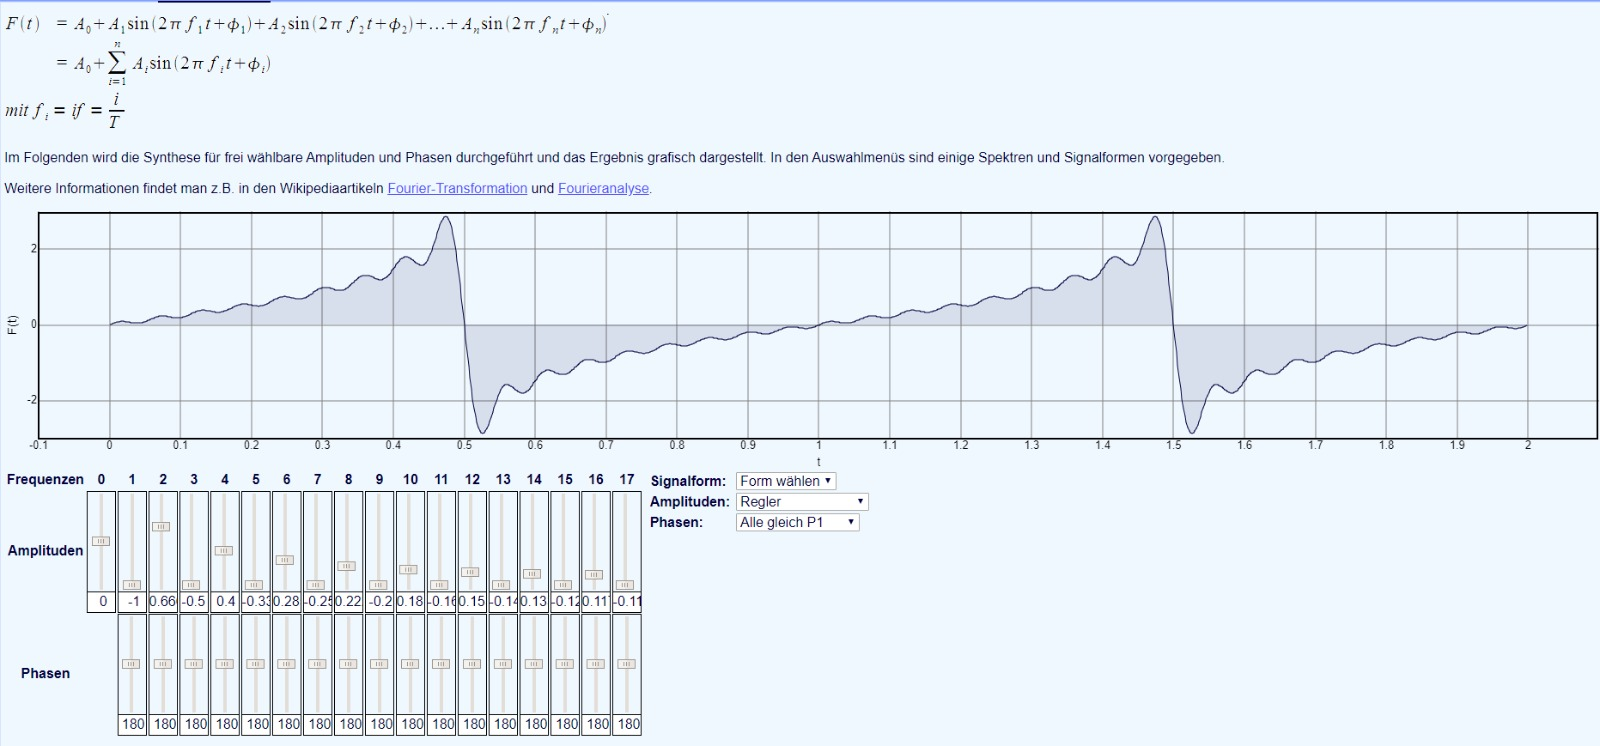
\includegraphics[width=\textwidth]{content/Fourier_x.png}
  \caption{Die Funktion mit eingesetzten Koeffizienten aud der \href{https://www.j-berkemeier.de/Fouriersynthese.html}{Website}}
  \label{fig:f(x)=x}
\end{figure}

\end{document}